\documentclass[upright, contnum]{umemoria}

%fix for the oneside argument
\makeatletter
\g@addto@macro\titlepage{\pagenumbering{Alph}}
\g@addto@macro\endtitlepage{\pagenumbering{roman}}
\makeatother

\depto{Departamento de Ciencias de la Computación}
\author{Daniel Alejandro Diomedi Pinto}
\title{Question Answering over Wikidata using Entity Linking and Neural Semantic Parsing}
\auspicio{}
\date{Octubre 2020}
\guia{Aidan Hogan}
\carrera{Ingeniero Civil en Computación y grado de Magíster en Ciencias, Mención Computación}
\memoria{Tesis para optar al Grado de \break Magíster en Ciencias, Mención Computación \break\break Memoria para optar al titulo de Ingeniero Civil en Computación}
\comision{}

\usepackage{lipsum}

\usepackage[utf8]{inputenc}
\usepackage[T1]{fontenc}

\begin{document}

\frontmatter
\maketitle

\begin{resumen}
    {\lipsum[1-4]}
\end{resumen}

\begin{abstract}
    {\lipsum[1-4]}
\end{abstract}

\begin{dedicatoria} % opcional
Una dedicatoria corta. Por ejemplo, al \emph{Centro Tecnológico Ucampus}
\end{dedicatoria}

\begin{thanks} % opcional
\lipsum[1-2]
\end{thanks}
\cleardoublepage

\tableofcontents
\listoftables % opcional
\listoffigures % opcional

\mainmatter
% Introduccion
\begin{intro}
	%   Motivacion
	\section{Motivation}
The volume of knowledge found on the web is growing considerably, so the interest of many 
communities is in profiting from that knowledge. Many questions are being asked  
to search engines like Google, which serves roughly 4.2 million searches done by users every 
minute\footnote{\href{https://www.internetlivestats.com/}{https://www.internetlivestats.com/}}. 
Since most of the data found on the web does not have a standard structure, 
search engines do not tend to reply to the question directly but just to retrieve the documents 
that might contain the answer. Though many questions can be answered by doing so, many 
other more complex questions require a higher level of reasoning that is difficult to achieve 
by consulting only unstructured data. Thus, there is still a challenging problem with making 
data more accessible, even knowing that its volume is increasing exponentially.
% \href{https://www.internetlivestats.com/}{Internet Live Stats - Internet Usage \& Social Media Statistics}

To give semantic meaning to all this information available on the Web in a manner in which both 
humans and machines can understand, a common framework is required. Thus, 
the Semantic Web~\cite{key:semwebsa} was proposed as an extension of the World Wide Web built on 
standards set by the World Wide Web Consortium (W3C). The primary purpose of this 
initiative is to support a \dquotesit{Web of Data} where data can be searched like in databases, but 
at the scope of the Web. The compilation of Semantic Web techniques and tools provides 
a framework where applications can query that data, draw inferences using vocabulary, etc. 
Thus, the ultimate goal is to extend the variety of tasks that computational systems can 
support, while developing trusted interactions over the network. 

The Semantic Web establishes a standard method to describe data using the Resource 
Description Framework (\RDF)~\cite{key:rdfprimer11}. This data model describes resources using 
statements of the form subject-predicate-object, also called triples, and can be represented as a 
directed edge-labelled graph. A collection of \RDF{} statements is known as a Knowledge Graph 
(KG)~\cite{key:ldbook}. Altogether, these KGs when linked together on the Web give shape to what is 
called the Linked Data Cloud~\cite{key:ldprinciples}: a large amount of interlinked \RDF{} datasets that 
comprise more than 30 billion \RDF{} triples. Among the most popular KGs, Wikidata~\cite{KG:wikidata} and 
DBpedia~\cite{KG:dbpedia} are huge and become more useful and accessible each day for research fields 
and applications~\cite{wikidata:usage-MalyshevKGGB18, EL:dbpedia-spotlight-MendesJGB11}. 

Wikidata~\cite{KG:wikidata} is a free open Knowledge Graph that can be read and edited by both humans 
and machines. Since the Wikimedia Foundation first launched Wikidata in October 2012, it has grown 
vastly. It has served as a reference resource for many of Wikimedia’s sister 
projects, like Wikipedia, the largest virtual encyclopedia on the Web. Wikidata is a valuable 
and comprehensive source of knowledge. It is supported mainly by its community and is 
designed in a way that people from all over the world can contribute. Many applications have 
used Wikidata as an information provider such as Apple’s Siri; it has also been used for research 
activities in life sciences and social science, and it even is used by Google to empower its search 
engine~\cite{wikidata:usage-MalyshevKGGB18}.

Thereafter, for querying this vast amount of data available on the web, a query language is needed. 
\SPARQL{}~\cite{key:sparql11} is a query language able to retrieve and manipulate data stored in \RDF{} 
format. The main advantages of \SPARQL{} are that it allows for writing queries that follow \RDF{} 
specifications and provides a specific graph transversal syntax for querying arbitrary-length paths 
in graphs.

While all of this knowledge available in the public domain drives growing interest in doing 
research regarding the Semantic Web, there is also a need to have a basic understanding of 
how data is structured (\RDF) and how to access this data (\SPARQL). These requirements 
represent a barrier-to-entry for non-expert users. Hence these barriers lead to the broad and 
complex challenge of developing intuitive and easy-to-use interfaces for end-users.

Many solutions have emerged to approach this issue, among which natural language interfaces such as 
Question Answering Systems (QASs)~\cite{qa:survey-BOUZIANE2015366, qa:intro-UngerFC14, 
qa:nn-qakg-Chakraborty19} have been receiving much attention. These systems aim to answer questions 
posed by humans in natural language, extracting the answer from one or more sources. There are QASs 
able to retrieve answers from an unstructured collection of natural language~\cite{qa:survey-BOUZIANE2015366}. 
However, we are interested in systems able to construct their responses by querying structured data, 
like relational databases or knowledge graphs from the Linked Data Cloud.

More specifically, the task of answering natural language questions using Knowledge Graphs 
is known as Question Answering over Knowledge Graphs (KGQA)~\cite{qa:nn-qakg-Chakraborty19} or Question 
Answering over Linked Data (QALD)~\cite{qa:intro-UngerFC14, qa:qald-Lopezetal2013}. Unger et 
al.~\cite{qa:intro-UngerFC14} define the QALD task as follows: \dquotesit{translate the users’ 
information need into a form such that they can be evaluated using standard Semantic Web query 
processing and inference techniques}. Their work also describes the types of questions these systems 
aim to answer, which often focus on definition questions (\dquotesit{Who was Tom Jobim?}) or factoid 
questions. These last ones that can be divided into predicative questions (\dquotesit{Who was the 
first man in space?}), list questions (\dquotesit{Give me all cities in Germany}) or boolean questions 
(\dquotesit{Was Margaret Thatcher a chemist?}). 

Several Question Answering systems have been developed to address some of the main 
challenges in Question Answering, commonly using pattern matching~\cite{qa:pattern-FaderZE13, 
qa:pattern-LopezFMS12}, grammar-based techniques~\cite{qa:grammar-DamljanovicAC10, 
qa:grammar-2-Marginean17}, or graph exploration~\cite{qa:graph-XuFZ14, qa:graph-2-ZouHWYHZ14} 
approaches. Although these systems have shown good results when dealing with a considerable amount of 
questions, their performance decreases~\cite{qa:challenges-semweb-HoffnerWMULN17} with questions 
involving more complex graph patterns or with vocabulary mismatches caused by the user typing 
different terms to the ones contained in the Knowledge Graph from which the information is being 
retrieved (this issue is also known as the lexical gap~\cite{semPar:lexical-gap-HakimovUWC15}). One 
example is the question \dquotesit{Which US player is the highest scorer in World Cups?} which could 
require complex operations like aggregation and sorting (count goals, sort and retrieve the maximum 
scorer) and might have vocabulary mismatches (it is not made explicit that we refer to FIFA World 
Cups, or the US might not be registered as an abbreviation of United States).

Aside from works that have tried to mitigate these problems~\cite{semPar:lexical-gap-HakimovUWC15, 
semPar:complex-queries-GliozzoK12}, some approaches that rely on Semantic Parsing have shown positive 
results due to recent advances in Deep Learning applied to Natural Language 
Processing~\cite{semPar:sempar-as-mt-AndreasVC13}. Semantic Parsing is the process of mapping a 
natural language sentence into a formal representation of its 
meaning~\cite{semPar:sempar-as-mt-AndreasVC13}. Some applications include code 
generation~\cite{semPar:code-gen-RabinovichSK17, semPar:tranx-code-gen-YinN18}, automated 
reasoning~\cite{semPar:ITPKaliszykUV17} or query construction~\cite{semPar:txt-to-sql-RadevKZZFRS18}. 
In particular, Andreas et al.~\cite{semPar:sempar-as-mt-AndreasVC13} discussed how Semantic Parsing 
could benefit from using Machine Translation methods, whereby natural language is \dquotes{translated} 
into a structured representation. Following their work, some Neural Machine Translation (NMT) approaches 
have brought about a growing interest in applying deep neural networks to Semantic Parsing 
problems~\cite{nmt:CaiXZYLL18, nmt:DongL16, nmt:ZhongCoRR17}. In NMT, pairs of sequences are given as 
input to a Deep Neural Network model, which is expected to learn the translation model. A natural idea 
is then to try to apply the NMT approach for translating Natural Language (NL) to \SPARQL{}, and some 
works have begun to explore such techniques~\cite{nmt:CoRRLuz18, nmt:nspm-SoruMMPVEN17, nmt:CoRRSoru18}.

There are multiple challenges relating to converting a NL question to its \SPARQL{} query 
representation (\NLtoSPARQL); some of these challenges are directly inherited from the 
original NL-to-NL translation problem, while others are distinct. First, there isn’t a one-to-one 
mapping for every NL question to a \SPARQL{} query. On one hand, there are multiple ways to 
express a question in NL. For example, the question \dquotesit{How far away is the Earth from the Sun?} 
can also be rephrased as \dquotesit{What is the distance between the Sun and Earth?}. On the other 
hand, questions can be translated to \SPARQL{} in different ways. For example, a question \dquotesit{What 
is the largest country in Africa?} might be translated to a query based on population or area, 
where one such translation must be chosen, and where both give different answers. Moreover, 
one \SPARQL{} query has potentially equivalent queries that will return the same results (over any 
data). In the question about US players, for example, we can first retrieve US players and then 
count their scores, or vice versa; thus there is a need to establish some common conventions 
when designing \NLtoSPARQL{} systems. 

Another issue is the lack of corpora for training \NLtoSPARQL{} models when compared to 
the enormous amount of documents in different languages that can be found on the Web for 
training \texttt{NL-to-NL} models (e.g. news, blogs, articles, academic documents, etc.). Generating 
data for \NLtoSPARQL{} is not an easy task considering the need for a basic \SPARQL{} understanding 
to build such datasets, although there is some work regarding automating parts 
of the process of generating \NLtoSPARQL{} pairs~\cite{dataset:dbnqa-hartmann-marx-soru-2018, 
dataset:lcquad-TrivediMDL17}. Furthermore, the queries required to answer a question change from 
dataset to dataset, where the \SPARQL{} queries needed for DBpedia are not the same as those for Wikidata.

One of the most recent works in regards to using NMT for \SPARQL{} is that 
the \textit{Neural SPARQL Machine} (NSpM)~\cite{nmt:nspm-SoruMMPVEN17}, which considers \SPARQL{} as a foreign 
language. The main idea is to train an end-to-end learning model to translate any NL expression 
into a sequence of tokens in the \SPARQL{} grammar that expresses a query equivalent to the 
question over a given dataset. Question Answering systems based on neural networks usually 
aim to generate the whole \SPARQL{} query in an attempt to perform the entire process of 
identifying the relevant entities along with deducing the KG properties, triples, and operators 
that would retrieve the expected answer. 

An analysis of the performance of many NMT models on translating NL to \SPARQL{} 
has been performed by Yin et al.~\cite{nmt:nl-to-sparql-Yin19}, where eight deep neural network models 
were tested over different datasets based on questions over DBpedia. One relevant dataset is the 
\textit{Large Complex Question Answering Dataset} (\LCQuADone)~\cite{dataset:lcquad-TrivediMDL17}, 
consisting of 5,000 complex questions based on 38 hand-made templates. Another dataset is the 
\textit{DBpedia Neural Question Answering} dataset (\DBNQA)~\cite{dataset:dbnqa-hartmann-marx-soru-2018} 
that includes almost 900,000 questions based on templates extracted from questions of the \LCQuADone{} 
dataset and the 7\textsuperscript{th} version of the \textit{Question Answering over Linked Data} 
dataset (\QALDseven)~\cite{dataset:qald7-UsbeckNHKRN17}.

Though the performance of these models shows promising potential for constructing meaningful 
and useful \SPARQL{} queries, they present some key limitations relating to the data 
used to train the models. First, despite the fact that many NMT models report positive results 
when evaluated over simple and large datasets like the \DBNQA{} dataset~\cite{nmt:nl-to-sparql-Yin19}, 
which contains questions with little variation in syntax and phrasing, such regular data do not give 
an accurate understanding of the real performance of these systems. In fact, the performance of such 
models drops dramatically when evaluated over more complex questions like the ones included in the 
\LCQuADone{} dataset, which might not contain enough questions to learn 
accurately~\cite{nmt:nl-to-sparql-Yin19}. Second, the current models are vocabulary-dependent, which 
means there is no capability for recognizing new entities or properties that were not used in the 
training data~\cite{nmt:nl-to-sparql-Yin19}. These issues lead to the constant need to train the model 
with new, manually created pairs of NL questions and \SPARQL{} queries.

The first issue can be addressed by building a more comprehensive dataset that has enough 
cases for an NMT to learn properly while maintaining an abstraction level that allows us to 
respond accurately to complex and diverse questions. Regardless, creating new datasets does 
not necessarily help with the vocabulary dependency issue, unless we have examples using 
every entity and property in the Knowledge Graph, which seems infeasible to generate in the 
short-to-medium term. Therefore, an important goal is to maximize the available training examples, 
where there is a need to find an alternative approach to complement the parsing power 
of NMTs with a system that helps to address vocabulary dependency by extracting the 
information NMTs cannot generalize.

For example, NMTs cannot be expected to extract entities from a question and translate them to their 
identifiers in the KG. Developing labelled examples for each entity does not seem feasible, as 
mentioned before. Plenty of solutions have addressed the entity extraction task over Linked Data. In 
particular, the Information Extraction area, which involves the automatic extraction of implicit 
information from unstructured or semi-structured sources, intersects in many ways with the 
Semantic Web~\cite{infExtr:MartinezHL19}. Some examples are systems that perform Named Entity 
Recognition~\cite{ner:LampleBSKD16}, Sequence Labeling~\cite{seqlab:MaH16, 
seqlab:contextual-emb-AkbikBV18}, or Entity Linking~\cite{EL:dbpedia-spotlight-MendesJGB11, 
EL:aida-tool-YosefHBSW11, EL:tagme-FerraginaS10, EL:opentapioca-Delpeuch19} while leveraging Semantic 
Web resources and/or techniques. In particular, Entity Linking (EL) systems aim to perform the entire 
process of identifying entity names in a text, mapping names to KG resources, and disambiguating them 
depending on the context of a given corpus~\cite{EL:survey-WuHH18}. Considering again the question 
\dquotesit{Which US player is the highest scorer in World Cups?}, an EL system could effectively 
identify the resources associated with the country US or the FIFA World Cup. Many EL 
systems~\cite{EL:dbpedia-spotlight-MendesJGB11, EL:aida-tool-YosefHBSW11, EL:tagme-FerraginaS10, 
EL:opentapioca-Delpeuch19} have achieved positive results when linking entities over text and 
these systems tend to generalize well over any new corpus. 

Furthermore, these Information Extraction tools can be complemented with intermediate 
representation of structured queries. An example can be found in a proposed 
Text-to-SQL system~\cite{semPar:txt-to-sql-RadevKZZFRS18}, where given a question in NL, an 
intermediate representation of an \SQL{} query is generated, consisting of a \SQL{} template with slots to 
be filled later with relevant words identified in the question using Named Entity Recognition 
tools~\cite{ner:dynet-NeubigDGMAABCCC17}.

We see an opportunity to improve state-of-the-art performance for QASs in the context 
of \RDF/\SPARQL{} by exploring the idea of combining the parsing capacity of NMT to get an 
intermediate representation of a \SPARQL{} query, with the entity extraction and disambiguation 
power of Entity Linking systems to identify the relevant entities in questions, decreasing 
the dependency of current QA systems on training examples that cover the full vocabulary of a 
Knowledge Graph. Additionally, there are many challenges to address – as we have previously mentioned 
– like how to deal with different representations of the same question (e.g. paraphrased questions), 
what canonical representation of \SPARQL{} queries we should adopt, how to evaluate 
that a QAS is fulfilling its purposes, among others.	
	%   Hipotesis, Objetivos, Metodologia
	\section{Hypothesis}
In this work, we propose the following hypothesis: \dquotesit{a combination of Information 
Extraction with Semantic Parsing can develop a Question-Answering system that outperforms 
a system that relies only on Semantic Parsing in the Question Answering over Knowledge 
Graphs task}.

In order to measure performance, this work will use metrics based on two perspectives: 
one focuses on the final answers that are derived from Question Answering over Knowledge 
Graphs (KGQA) benchmarks (i.e., a Question Answering-based evaluation), and the second 
focuses on how close is the generated \SPARQL{} query compared with the expected query (i.e., 
a Machine Translation-based evaluation).

The scope of this work will be limited to answering questions in English, but similar 
techniques should be applicable in any other language assuming the availability of similar 
datasets for that language. In the same way, this hypothesis will be explored in the context of 
questions over Wikidata, so the results might differ for other Knowledge Graphs. Nevertheless, 
the selected approach should be generalizable to other domains. 

\section{Objectives}
\subsection*{General Objective}
% \lipsum[1-3]
We aim to improve upon state-of-art Question Answering systems 
based on Neural Semantic Parsing models by reducing vocabulary dependency on the 
data used in the learning process of such models.
\subsection*{Specific Objectives}
% \lipsum[1-3]
The specific objective is to build a Question-Answering system over Wikidata in English, 
that relies on Entity Linking and Neural Machine Translation systems, with an intermediate 
system that combines both tools. Our initial claim is that such a system can improve upon 
the state-of-the-art Neural Machine Translation approaches found in the literature.  

\section{Methodology}
Accomplishing the proposed objectives involves the following tasks:
\begin{itemize}
    \item Survey previous work regarding Neural Machine Translation, Entity Linking, and 
    Question Answering approaches that rely on Neural Machine Translation.
    \item Define a benchmark that should include KGQA datasets for training, validation and 
    testing along with metrics to compare all involved systems.
    \item Define a baseline system for Question Answering based on Neural Machine Translation.
    \item Define a pipeline process to convert a natural language question into a \SPARQL{} query 
    by combining Entity Linking techniques with Neural Machine Translation.
    \item Implement a Question-Answering system over Wikidata in English based on the designed pipeline.
    \item Validate the proposed system by comparing it with baseline approaches over the 
    proposed benchmark.
\end{itemize}
	
	% 	Contribuciones
	\section{Contributions}
\label{cap1:intro/contributions}
% \lipsum[1-3]
We present the three main contributions anticipated for this work.
\subsection*{Benchmark on Question Answering over Wikidata}
After a bibliographic revision, we will define a benchmark as a combination of three 
components: a baseline system, a set of metrics to compare with the baseline, and one or 
more datasets with which to conduct experiments.

The baseline consists of one of the Neural Machine Translation systems described by 
Yin et al.~\cite{nmt:nl-to-sparql-Yin19}. From the eight models that were compared in this work, 
the ConvS2S model~\cite{nmt:convS2S-GehringAGYD17} 
significantly outperforms all the other models . Following these results, a baseline QAS is 
implemented using the Fairseq library~\cite{nmt:fairseq-OttEBFGNGA19}, which includes a ConvS2S implementation over 
Pytorch\footnote{\url{https://pytorch.org/}} ready to use for training and translation. The model is trained using the same 
settings described by Yin et al.

The primary dataset used is the \LCQuADtwo{} dataset, which contains around $30,000$ 
questions over Wikidata~\cite{dataset:lcquad2-DubeyBA019}. A quality check is performed over this dataset, where cases 
that contain either invalid questions or invalid \SPARQL{} queries are filtered. The \DBNQA{} 
dataset~\cite{dataset:dbnqa-hartmann-marx-soru-2018} is considered as well, where a mapping process is applied to obtain queries over 
Wikidata. The queries that cannot be mapped are ignored. The Question Answering over 
Linked Data (QALD)~\cite{qa:qald-Lopezetal2013} dataset is also used as part of this benchmark. In particular, the 
150 questions included in \QALDseven{}~\cite{dataset:qald7-UsbeckNHKRN17} that can be answered over Wikidata are considered. 
Besides these datasets, we build a new dataset of 100 questions over Wikidata. Only \LCQuADtwo{} 
and the mapped version of \DBNQA{} are used for training and validation. The other 
datasets are used only for testing purposes. All datasets are arranged to follow a common 
format, which will permit an easy evaluation of every subtask performed for the proposed 
Question Answering system (Entity Linking, Query Template Generation, Slot Filling) along 
with the main task (Question Answering over Knowledge Graphs).

The metrics used for comparing systems are based on the ones used for comparing Neural 
Machine Translation systems and the ones found on the QALD benchmark. The first set of 
metrics includes the BLEU score, Perplexity, and Accuracy by comparing an exact match on 
the \SPARQL{} query. On the other hand, the QALD benchmark uses Precision, Recall, and F1-score 
over the answers obtained when executing the output \SPARQL{} query. Additionally, 
we propose a fine-grained analysis over each case where predicted queries are evaluated with 
respect to the following components: correct entities, correct slots, and correct query 
templates.

\subsection*{Question Answering system over Wikidata}
\label{cap1:intro/contributions/qaWikidata}

The main contribution of this work is a Question Answering system that translates 
natural language questions in English to \SPARQL{} queries executable on Wikidata endpoints. See an
example of an expected \SPARQL{} query in Figure~\ref{fig:introQAexample}. The implementation of this 
system is divided into the construction of three modules: a Query Template generator, 
an Entity Linking system, and an intermediate Slot Filling system. 

\begin{figure}[!h]
    \centering
    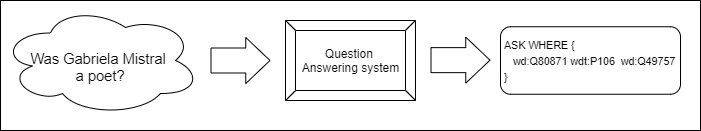
\includegraphics[scale=.5]{imagenes/1_intro/introQuestionAnsweringExample.png}
    \caption{Expected \SPARQL{} query example from a KGQA system.}
    \label{fig:introQAexample}
\end{figure}

The Query Template generator produces incomplete \SPARQL{} queries (which we call 
Query Templates) that contain \dquotesit{placeholders} in the position where entities are 
supposed to be (e.g. placeholders \texttt{<sbj\_1>} and \texttt{<obj\_1>} instead of entities 
\texttt{Q80871} and \texttt{Q49757} of the query shown in Figure~\ref{fig:introQAexample}). 
This module is built using the same model used to implement the baseline QAS. 
However, the training data is adapted to generate Query Templates instead of the complete 
query. This is achieved by removing the entities from the output \SPARQL{} queries included 
in the selected datasets such that the entities can rather be found by Entity Linking.

The role of the Entity Linking module is to recognize the relevant entities contained
in each question (e.g. identify that concepts \dquotesit{Gabriela Mistral} and \dquotesit{poet}
corresponds to the entities \texttt{Q80871} and \texttt{Q49757} in Figure~\ref{fig:introQAexample}) 
that are used to fill the Query Template. We implement various entity retrieval systems using 
one or more of the existing Entity 
Linking systems that have APIs available. The first variant is to use each EL system individually, 
which includes DBpedia Spotlight~\cite{EL:dbpedia-spotlight-MendesJGB11}, AIDA~\cite{EL:aida-tool-YosefHBSW11}, 
TAGME~\cite{EL:tagme-FerraginaS10}, and OpenTapioca~\cite{EL:opentapioca-Delpeuch19}. 
All of these systems, except for OpenTapioca, only work for DBpedia; therefore an 
extra mapping layer is implemented to map DBpedia entities to Wikidata entities. Two ensemble 
EL approaches are then proposed: one that prioritizes systems with higher Precision 
and another that implements a voting mechanism. We keep the variant that performs best 
according to the experiments that are explained in the \textit{Experimental results} subsection.

Additionally, a Slot Filling module is built by combining a Sequence Tagger model of the Flair 
library~\cite{seqlab:flair-AkbikBBRSV19} and a filling algorithm proposed in this work. Training 
the Sequence Tagger model requires building training data based on the selected datasets. 
Intuitively speaking, a Query Template may have multiple slots and multiple entities, where the 
Slot Filling module decides which entity should fill which slot (e.g. to infer that the concept 
\dquotesit{Gabriela Mistral} corresponds to the placeholder \texttt{<sbj\_1>}, therefore the 
entity \texttt{Q80871} should replace the occurrences of \texttt{<sbj\_1>} in the Query Template).

\subsection*{Experimental results}
\label{cap1:intro/contributions/expResults}
We conduct several experiments for validating each implemented module (Entity Linking, 
Slot Filling, and Query Template Generation) along with experiments over the defined 
benchmark for the end-to-end Question Answering process.

The Entity Linking systems are compared using Precision, Recall, and F1-score on the 
entities for each case on the dataset used for training. Testing is conducted over \QALDseven{} and 
our proposed dataset. The slot filling system is validated using Precision, Recall, and F1-score 
over the identified BIO labels (a common tagging format for sequence labeling tasks) over 
\LCQuADtwo{} and the mapped \DBNQA{} dataset. The query generator system is validated 
using BLEU score, Perplexity, and Accuracy over \LCQuADtwo{} and the mapped \DBNQA{} 
dataset. When training the query generator system, many split methods are tested according 
to the methodology proposed by Finegan-Dollak et al.~\cite{semPar:txt-to-sql-RadevKZZFRS18} for Text-to-SQL systems. 
The end-to-end Question Answering system is tested over all the datasets using the metrics 
described in the \textit{Benchmark on Question Answering over Wikidata} subsection.	
	%   Estructura del trabajo
	\section{Work Structure}
This worked is divided into the following chapters:

\begin{enumerate}
    \item In Chapter~\ref{cap2:theoFrame}, we describe the theoretical framework 
    enclosed on this work. This chapter covers concepts about what is the Semantic 
    Web, Information Extraction methods and how they relate with Semantic Web 
    technologies, Semantic Parsing applied on translating natural language to 
    \SPARQL, and the current state and challenges of the Question Answering over 
    Knowledge Graphs task.
    \item In Chapter~\ref{cap3:system}, we give an overview of the proposed Question 
    Answering system for this work. This includes a general explanation on the 
    pipeline proposed to generate a SPARQL query, and more specific details on how 
    each component is designed.    
    \item In Chapter~\ref{cap4:experimentalDesign}, we go into details about the 
    experiments we run on this work. We present the research questions we aimed to answer, 
    the baseline we compare our system with, and the metrics used to quantify the 
    performance of each system.    
    \item In Chapter~\ref{cap5:results}, we present the results derived from running the 
    proposed experiments. Aside from that, we include a brief discussion and analysis of 
    the results.    
    \item In Chapter~\ref{cap6:conclusions}, we summarize the conclusion of this work, 
    discuss its limitations and the future work regarding Question Answering over 
    Knowledge Graphs.
    
\end{enumerate}
	
\end{intro}
% Marco teorico
%   RDF y SPARQL
%   Redes Neuronales
%   Slot Filling
%   Entity Linking
%   Question Answering
% Trabajo relacionado
% Baseline
% Sistema propuesto
%\input{cap1.tex}
%\chapter{Segundo}
\lipsum[1-3]
    \lipsum[30-35]
	\begin{enumerate}
		\item Item 1
		\begin{enumerate}
			\item Subitem 1
			\item Subitem 2 (ver Figura \ref{logofcfm})
		\end{enumerate}
		\item Item 2
		\item Item 3
	\end{enumerate}
	\begin{teo}
	Se tiene que $$\int_0^t e^sds=e^t-1.$$
	\end{teo}
	\lipsum[36-40]
\begin{defn}[ver \cite{rdf}] Definición definitiva $$\frac{d}{dx}\int_a^xf(y)dy=f(x).$$\end{defn}
\lipsum[50-60]
%\input{conclu.tex}

% \input{glosario.tex} % opcional

\bibliographystyle{plain}
\bibliography{bibliografia}

% \input{anexo_apendices.tex} % opcionales

\end{document}
